Neste capítulo, detalha-se o estágio atual do projeto e o planejamento para a conclusão da dissertação. Como esta proposta é apresentada em um estágio avançado do mestrado, a fase de construção do artefato (aplicação \textit{web}, \textit{backend} e integração com IA) já se encontra concluída (Fase de Design e Desenvolvimento), permitindo que os esforços futuros se concentrem na validação científica (Fase de Avaliação) e na escrita final.

\section{Estágio Atual do Desenvolvimento}

Sob a ótica da \textit{Design Science Research}, o artefato computacional proposto já atingiu um nível de maturidade funcional que permite a execução de testes. As seguintes etapas do ciclo de pesquisa foram concluídas:

\begin{itemize}
    \item \textbf{Identificação do Problema e Motivação:} Mapeamento das dificuldades de acesso aos dados brutos do Senado Federal e definição da relevância para o controle social e participação democrática.

    \item \textbf{Definição da Solução:} Projeto de uma arquitetura baseada em Dashboard (visualização) + Chatbot (interação conversacional) para reduzir barreiras cognitivas ao acesso legislativo.

    \item \textbf{Design e Desenvolvimento:} Implementação completa dos módulos de coleta (ETL via API Senado), análise (Mistral 7B Instruct em ambiente local) e interface (\textit{Streamlit} com \textit{Plotly}), resultando em um protótipo funcional capaz de processar dados reais.

    \item \textbf{Demonstração:} Validação técnica preliminar mostrando que o artefato consegue processar dados parlamentares e gerar respostas coerentes.
\end{itemize}

A aplicação encontra-se implantada em ambiente de homologação, processando dados da API do Senado Federal e respondendo a consultas em linguagem natural. Esse estágio habilita a fase de avaliação técnica do artefato, com foco em qualidade dos dados processados, acurácia da classificação temática, qualidade factual das respostas e rastreabilidade das informações geradas.

\section{Arquitetura e Componentes do Artefato}

\subsection{Camada de Dados: Coleta e Processamento}

A coleta de dados é efetuada via API de Dados Abertos do Senado Federal \cite{SenadoFederal_s_d}. O processo de ETL (\textit{Extract, Transform, Load}) é automatizado e inclui:

\begin{itemize}
    \item \textbf{Extração:} Utilização da biblioteca \textit{Requests} \cite{RequestsLib} para requisição de dados brutos (XML/JSON) dos \textit{endpoints} da API Swagger, mapeando informações sobre sessões legislativas, discursos, votações e senadores.

    \item \textbf{Transformação:} Conversão e limpeza dos dados utilizando \textit{Pandas} \cite{PandasLib}, normalizando formatos, removendo duplicatas, preenchendo valores ausentes e estruturando informações em tabelas relacionais otimizadas para análise.

    \item \textbf{Carregamento:} Os dados transformados são mantidos em memória durante a execução e persistidos em um \textit{cache} em arquivo (\texttt{outputs/materias\_cache.json}), que funciona como \textit{snapshot} local: requisições repetidas à API são evitadas quando o mesmo período legislativo já foi coletado, e esse \textit{snapshot} pode ser versionado para assegurar a reprodutibilidade da avaliação sobre um corpus congelado.
\end{itemize}

A atualização do corpus ocorre sob demanda, mediante reexecução do \textit{pipeline} para o período desejado; neste estágio de prototipação não há um agendamento automático em produção. Para fins de avaliação científica, adota-se deliberadamente um \textit{snapshot} congelado e versionado dos dados, de modo que os experimentos sejam reproduzíveis sobre exatamente o mesmo conjunto --- condição necessária para que o gabarito de referência permaneça estável entre execuções.

\subsection{Camada de Inteligência: Análise com Mistral 7B}

O núcleo analítico utiliza o modelo Mistral 7B Instruct \cite{MistralAI2024}, executado em ambiente local. A justificativa dessa escolha --- privacidade e soberania de dados, replicabilidade, custo e adequação de desempenho ---, bem como a comparação com modelos proprietários e com outros modelos abertos, foi apresentada na fundamentação teórica (Seção~\ref{subsec:escolha_modelo}) e não é aqui repetida.

Do ponto de vista de implementação, o modelo é servido localmente por um \textit{runtime} de inferência que expõe uma API compatível com o padrão OpenAI em \texttt{localhost} (na configuração de referência, o LM Studio em \texttt{http://localhost:1234/v1}). O artefato comunica-se com o modelo exclusivamente por essa interface local: nenhum dado legislativo é transmitido a servidores externos, de modo que a soberania de dados é preservada mesmo havendo uma camada de \textit{serving} compatível com OpenAI. Essa padronização da interface é também o que torna o componente de linguagem modular e substituível por outro modelo sem alteração dos demais estágios.

O modelo é utilizado para duas funções críticas:

\begin{itemize}
    \item \textbf{Classificação Temática:} Engenharia de \textit{prompts} estruturados instrui o modelo a categorizar discursos legislativos em temas predefinidos (Saúde, Educação, Infraestrutura, Segurança, etc.). A classificação permite organização e análise dos debates por assunto.

    \item \textbf{Motor de Resposta (Recuperação Estruturada com Geração Aumentada):} O módulo recebe perguntas do usuário em linguagem natural via Chatbot, recupera da base em memória um subconjunto de registros relevantes à pergunta (busca estruturada por palavras-chave sobre os dados mantidos em cache de sessão) e instrui o Mistral 7B a gerar respostas contextualizadas e didáticas, fundamentadas nesses registros e citando-os por identificador estável (por exemplo, \texttt{[D1]} para discursos e \texttt{[V1]} para votações).
\end{itemize}

\subsection{Camada de Apresentação: Interfaces Acessíveis}

Para materializar o acesso democrático aos dados, desenvolveu-se uma interface \textit{web} utilizando o \textit{framework Streamlit} \cite{Streamlit2024}, oferecendo dois modos de interação complementares:

\subsubsection{Dashboard Visual}

Gráficos interativos gerados com \textit{Plotly} \cite{Plotly2024} permitem exploração visual de tendências legislativas. O design segue o mantra de Shneiderman \cite{Shneiderman1996}: "primeiro o panorama geral, depois zoom e filtros, e então detalhes sob demanda".

\textbf{Exemplos de visualizações disponíveis:}

\begin{itemize}
    \item Tendências de votação ao longo do tempo (linha temporal)
    \item Distribuição de votos por tema (gráfico de barras)
    \item Padrões de voto de senadores específicos (matriz ou radar)
    \item Comparação entre posições de diferentes grupos parlamentares (gráficos comparativos)
\end{itemize}

O Dashboard permite que usuários explorem livremente, filtrem por tema, senador ou período, e identifiquem padrões visuais em dados legislativos.

O uso do Streamlit é uma escolha compatível com o estágio de prototipação científica do artefato, pois permite rápida construção de interfaces interativas para análise de dados. Entretanto, reconhece-se que o framework possui limitações para uso em produção em larga escala, especialmente em autenticação, controle fino de permissões, escalabilidade e separação entre camadas de serviço. Assim, neste trabalho, o Streamlit é tratado como tecnologia de prototipação e demonstração do artefato, não como decisão definitiva para implantação institucional.

\subsubsection{Chatbot Conversacional}

Interface de \textit{chat} que abstrai a complexidade dos dados legislativos, permitindo consultas em linguagem natural:

\textbf{Exemplos de perguntas que o usuário pode fazer:}

\begin{itemize}
    \item "Como votou o Senador [Nome] sobre educação?"
    \item "Qual foi o resultado da votação em [Projeto de Lei]?"
    \item "Quais são os temas mais debatidos em 2025?"
    \item "Como o partido [X] votou no projeto sobre saúde?"
    \item "Qual senador votou diferente de seu partido nesta votação?"
\end{itemize}

O Chatbot traduz perguntas em linguagem comum para operações sobre a base de dados em memória, recupera as informações relevantes e retorna respostas em linguagem natural acessível a cidadãos sem expertise legislativa ou tecnológica. A Figura \ref{fig:tela_chatbot} ilustra a interface conversacional em operação com dados reais do Senado Federal.

\begin{figure}[H]
    \centering
    \caption{Interface do Agente Conversacional (Chatbot) do AgentAI}
    \label{fig:tela_chatbot}
    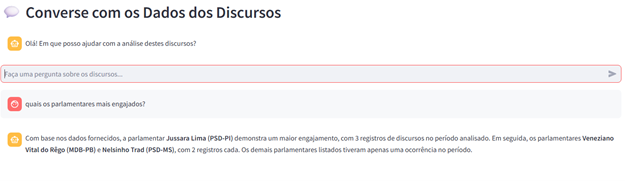
\includegraphics[width=0.9\textwidth]{imagens/tela_chatbot.png}
    \fonte{Produção da autora.}
\end{figure}

\subsection{Rastreabilidade das Respostas}

Para que o agente conversacional não opere como uma "caixa-preta", o artefato foi instrumentado de modo a tornar explícita a ligação entre cada resposta e os dados que a fundamentaram. Esse mecanismo, já implementado no protótipo, opera em dois níveis complementares:

\begin{itemize}
    \item \textbf{No artefato (rastreabilidade para o usuário):} a etapa de \textit{retrieval} seleciona, para cada pergunta, um subconjunto de registros da base e atribui a eles identificadores curtos e estáveis (\texttt{[D1]}, \texttt{[D2]}, \ldots\ para discursos; \texttt{[V1]}, \texttt{[V2]}, \ldots\ para votações). O \textit{prompt} instrui o modelo a fundamentar a resposta exclusivamente nesses registros e a citá-los por identificador, sendo vedado referenciar identificadores fora da lista recuperada. A interface exibe, junto a cada resposta, um painel "Fontes utilizadas" com a tabela dos registros efetivamente recuperados, preservando também o código oficial do Senado de cada item. O mecanismo aplica-se tanto ao \textit{chat} de discursos quanto ao de votações.

    \item \textbf{Para avaliação (instrumentação de medição):} cada consulta gera um registro estruturado em \textit{log} (arquivo \texttt{qa\_trace.jsonl}) contendo a pergunta, os identificadores das fontes recuperadas, os códigos oficiais correspondentes e a resposta gerada. Sobre esse \textit{log}, um módulo de avaliação calcula indicadores de rastreabilidade, também acessíveis por um painel dedicado na própria interface. Esse encadeamento --- recuperação, citação, registro e medição --- funciona de ponta a ponta; a medição sobre o conjunto de cenários definido, incluindo a verificação de suporte semântico das citações, integra a fase de avaliação ainda em execução, detalhada no Capítulo~\ref{cap:metodologia}.
\end{itemize}

\section{Fluxo de Funcionamento do Sistema}

O sistema opera conforme descrito abaixo:

\begin{enumerate}
    \item \textbf{Inicialização:} Aplicação \textit{Streamlit} carrega dados pré-processados da API do Senado Federal, mantendo-os em memória com cache de sessão.

    \item \textbf{Interação Usuário - Dashboard:} Usuário pode explorar Dashboard sem necessidade de entrada, aplicando filtros interativos para ver visualizações customizadas.

    \item \textbf{Interação Usuário - Chatbot:} Usuário digita pergunta em linguagem natural.

    \item \textbf{Processamento:}
    \begin{itemize}
        \item Sistema faz \textit{retrieval} de dados relevantes (busca estruturada por palavras-chave sobre a base local)
        \item Constrói contexto com os dados recuperados
        \item Instrui Mistral 7B com \textit{prompt} que inclui: pergunta do usuário, contexto de dados e instruções para responder de forma didática
    \end{itemize}

    \item \textbf{Resposta:} Mistral 7B gera resposta em linguagem natural, citando por identificador (\texttt{[D1]}, \texttt{[V1]}, etc.) quais registros recuperados foram utilizados.

    \item \textbf{Exibição:} A resposta é exibida no Chatbot, acompanhada do painel "Fontes utilizadas" que lista os registros recuperados. O usuário pode fazer pergunta de acompanhamento.
\end{enumerate}

\section{Dados Legislativos Utilizados}

O artefato processa dados da API de Dados Abertos do Senado Federal, incluindo:

\begin{itemize}
    \item \textbf{Senadores:} Nomes, partidos, estados, contatos
    \item \textbf{Sessões Plenárias:} Datas, tipo (ordinária, extraordinária, etc.)
    \item \textbf{Discursos:} Texto completo, senador autor, data, tema (quando disponível)
    \item \textbf{Votações:} Descrição da matéria votada, resultado, votos individuais de cada senador
\end{itemize}

Os dados cobrem o período de 2024 a 2026 e permitem a investigação de padrões legislativos contemporâneos. Esse recorte temporal poderá ser ampliado na etapa final da pesquisa, conforme a disponibilidade da API e os limites de processamento do ambiente local.

\section{Status de Conclusão das Fases DSR}

Conforme a metodologia Design Science Research (Cap.\ \ref{cap:metodologia}), o projeto encontra-se no seguinte estágio:

\begin{quadro}[H]
    \centering
    \caption{Progresso das Fases de Design Science Research}
    \label{quad:fases_dsr}
    \begin{tabular}{|p{4.5cm}|>{\centering\arraybackslash}p{2.8cm}|p{7cm}|}
        \hline
        \textbf{Fase DSR} & \textbf{Status} & \textbf{Descrição} \\
        \hline
        1. Identificação do Problema & Concluída & Problema definido, fundamentado em literatura \\
        \hline
        2. Objetivos da Solução & Concluída & Objetivos do artefato claramente especificados \\
        \hline
        3. Design e Desenvolvimento & Concluída & Artefato implementado e funcional \\
        \hline
        4. Demonstração & Concluída & Artefato operacional em ambiente de homologação \\
        \hline
        5. Avaliação & \textit{Em Execução} & Testes técnicos, factuais e de rastreabilidade planejados (Trim. 2-3) \\
        \hline
        6. Reflexão e Aprendizados & \textit{Planejada} & A executar após fase de avaliação (Trim. 3-4) \\
        \hline
    \end{tabular}
    \fonte{Produção da autora.}
\end{quadro}

\section{Cronograma de Execução da Dissertação}

O planejamento temporal das fases finais --- com foco na Avaliação rigorosa (Fase 5) e na produção textual até a defesa, prevista para janeiro de 2027 --- é apresentado de forma consolidada no Capítulo~\ref{cap:metodologia} (Quadro~\ref{quad:cronograma_metodologia}), evitando-se aqui a duplicação do cronograma. Esta seção registra apenas o encadeamento das próximas atividades imediatas, detalhado a seguir.

\section{Próximas Ações Imediatas (Próximas 8 Semanas)}

\begin{enumerate}
    \item Implementar melhorias apontadas pelo parecer de qualificação
    \item Finalizar dataset de controle para experimento de acurácia
    \item Preparar o conjunto de cenários representativos de consulta
    \item Executar primeira rodada de teste técnico (IA vs. Gabarito)
    \item Documentar detalhes finais do protocolo de avaliação técnica
\end{enumerate}
